\chapname = {MAAS in VENV - III : Nodes}

\chapter{\the\chapname}

\section{Creating a few nodes}

There is a restriction on creating virtual machine that it won't let you proceed until you specify an iso file. Hence, create a dummy iso file by using the command: 

\$ touch nothing.iso

We will start creating a single node and then we will clone that to make a few more nodes.

Configurations for creating a new virtual machine with dummy nothing.iso image:

\begin{itemize}
    \setlength\itemsep{0em}
    \item Memory - 1024 MB
    \item CPU Cores - 2
    \item Storage - 20 GB qcow2 
    \item Name - node0
    \item Boot order - 1.) PXE  2.) HDD
    \item Network - maasisotest
    \item NIC Interface 
    \begin{itemize}
        \item Network source - maasisotest
        \item Device model - virtio
    \end{itemize}
    \item Disk bus - virtio
    \item Remove unnecessary virtual hardware from the list for eg. sound
\end{itemize}

\begin{figure}[!ht]
    \centering
    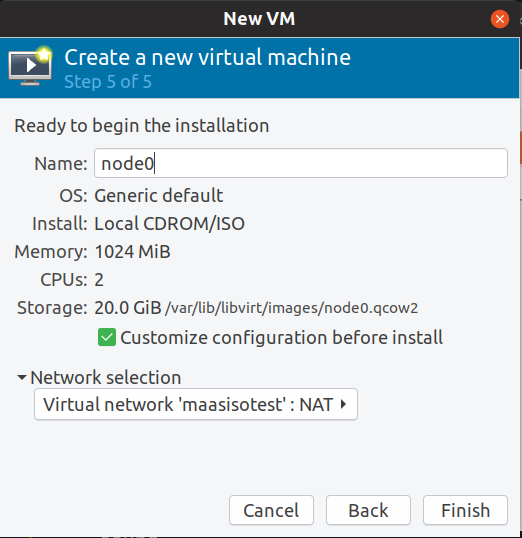
\includegraphics[width=0.5\textwidth]{images/5-1.png}
    \caption{Node 0}
\end{figure}


\begin{figure}[!ht]
    \centering
    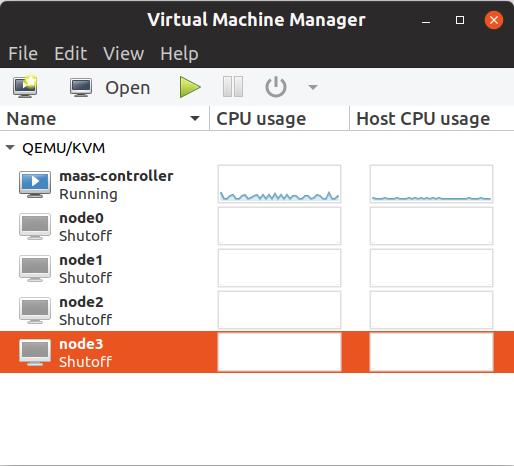
\includegraphics[width=0.5\textwidth]{images/5-2.png}
    \caption{Clones of node 0}
\end{figure}


Begin the installation and once the machine is open, pull the virtual power plug by force off, to create a few virtual machine clones.

Once the clones are created, power on all the virtual machines. These machines will boot for enlistment procedure. They will register themselves and shut themselves down.

\begin{figure}[!ht]
    \centering
    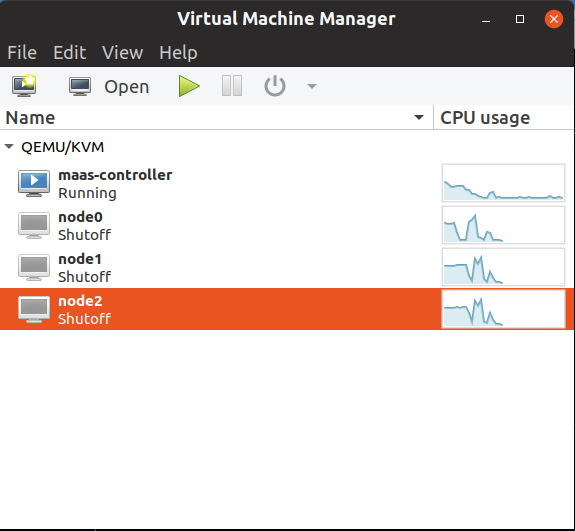
\includegraphics[width=0.5\textwidth]{images/5-3.png}
    \caption{Nodes enlisted themselves and shutdown}
\end{figure}

As soon as they shutdown, we will start confiiguring the power parameters. Before we do that, we need to change the identifications names of the nodes in the maas interface. To do this run the following command in the host:

\$ virsh dumpxml node0 | grep mac 

And then check for the device which has the same mac address in the maas interface and then set the name to node0. In the same way do for the other clones.

\begin{figure}[!ht]
    \centering
    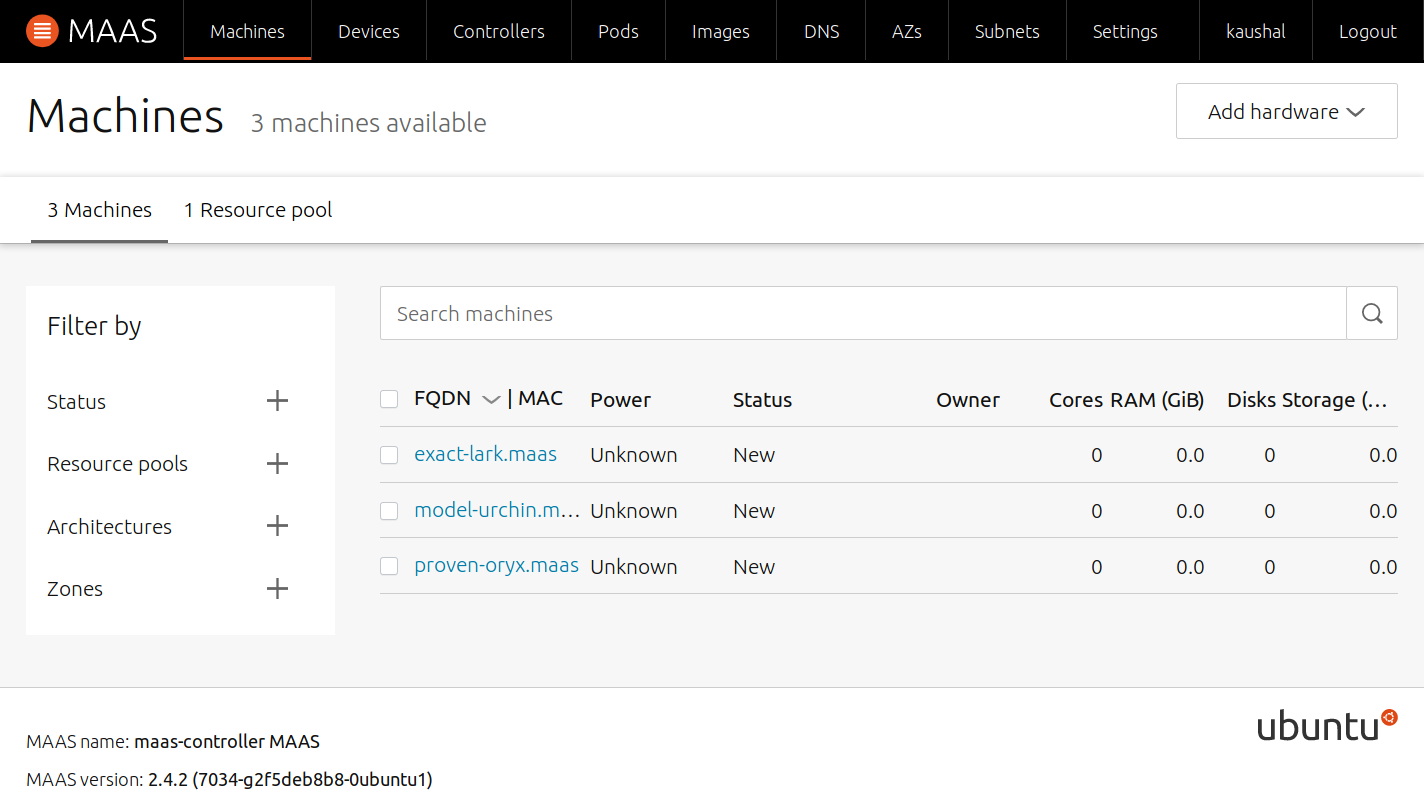
\includegraphics[width=0.7\textwidth]{images/5-4.png}
    \caption{Change these names to the meaningful names}
\end{figure}

Refer the Fig. 5.5 for power configuration of node0, likewise you need to configure power parameters for other nodes.

Power type: Virsh

Virsh Address: \url{qemu+ssh://kaushal@10.128.0.132/system}

Virsh VM ID: \url{node0}

\begin{figure}[!ht]
    \centering
    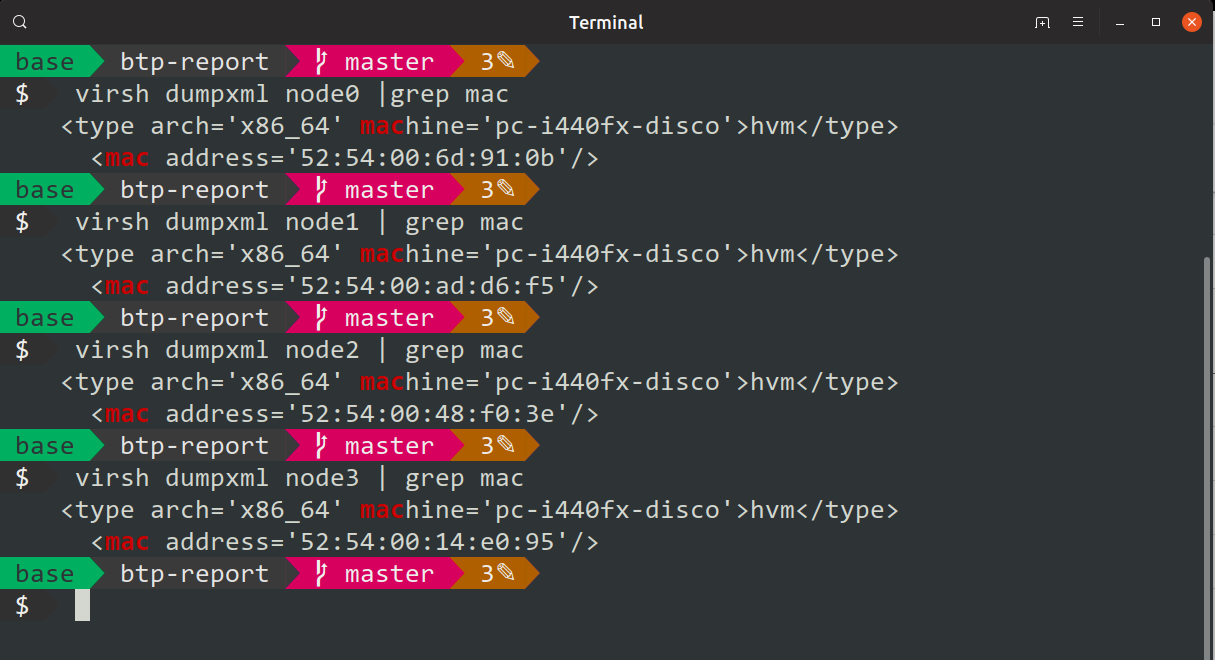
\includegraphics[width=0.7\textwidth]{images/5-5.png}
    \caption{Power configuration for node0}
\end{figure}

Once the power configuration is done select all nodes and commission all of them (fig 5.6). During the commissioning procedure the machine will also go through some hardware testing procedure (fig 5.7).

\begin{figure}[!ht]
    \centering
    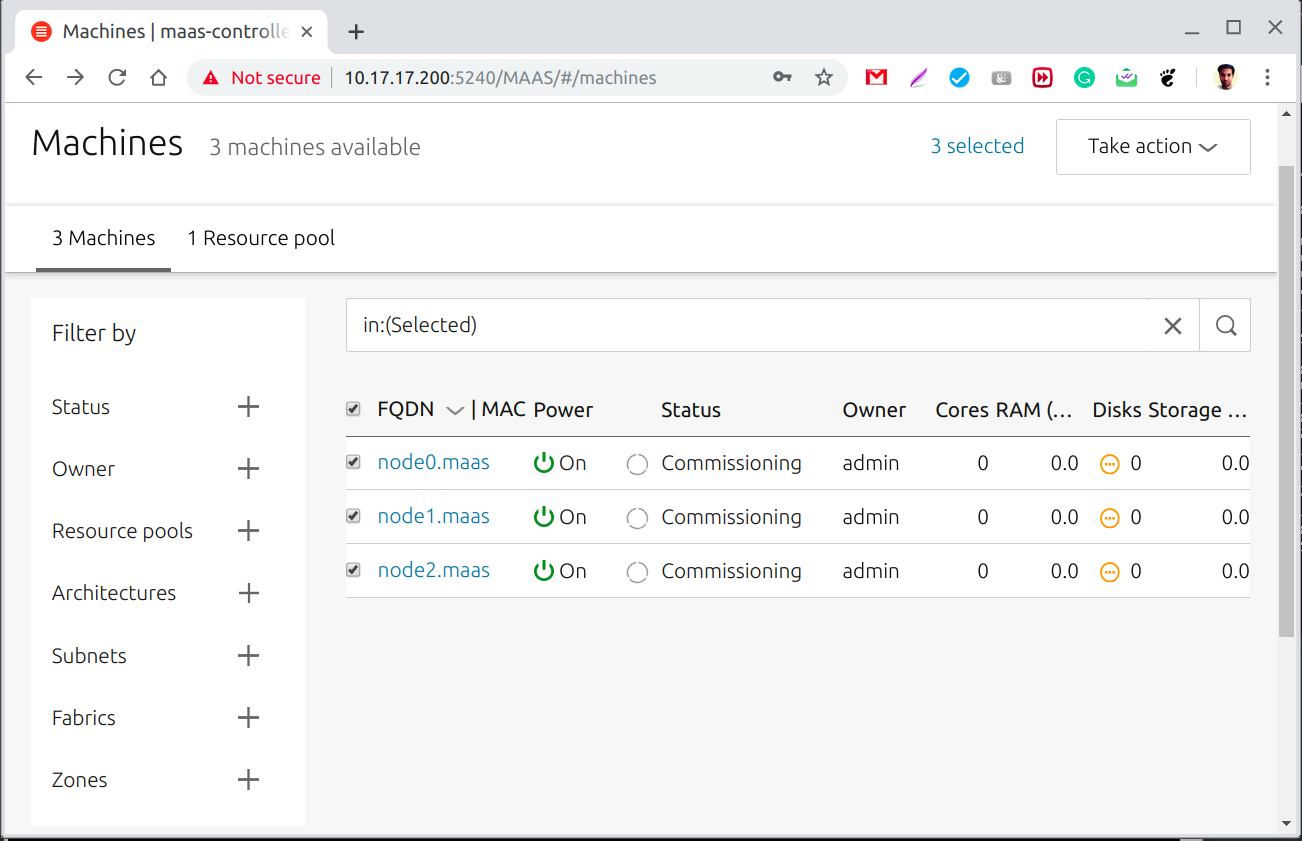
\includegraphics[width=0.7\textwidth]{images/5-6.png}
    \caption{Commissioning all nodes}
\end{figure}

\begin{figure}[!ht]
    \centering
    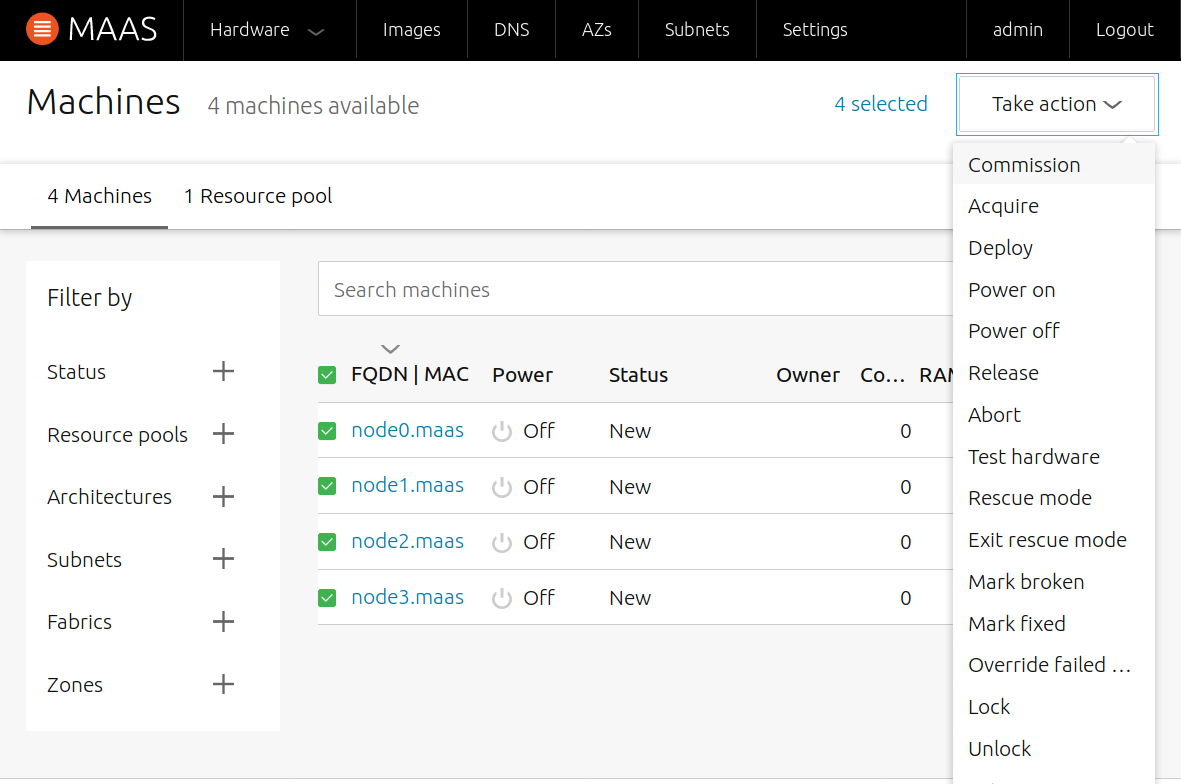
\includegraphics[width=0.7\textwidth]{images/5-7.png}
    \caption{Hardware testing phase}
\end{figure}

This is a basic procedure of how to create MAAS nodes and commission them.

In the next chapter we will discuss the node acquisition and deployment.